
\section{Résumé en français}
Le présent chapitre présente de façon détaillée le \textit{modèle d'océan} utilisé dans le cadre de ma thèse pour simuler numériquement les grandes échelles turbulentes (ou LES$^{\noparref{LES}}$) dans la région du détroit de Gibraltar mais aussi, plus généralement, pour développer des modèles analytiques simplifiés de processus au service de cette approche numérique. Plusieurs sections du chapitre ont été intégrées à des publications acceptées \citep{hilt_2020}, \citep{auclair_modied_2021} ou en cours de rédaction  \citep{auclair_NBQ1_2021} mais aussi au rapport d'études du programme amont PROTEVS Gibraltar du SHOM \citep{auclair_modelisation_2019}. L'ensemble du chapitre est par conséquent rédigé en anglais.

Dans une première partie (\S \noparref{section_prim_eq}) sont introduites les équations de conservations usuelles de l'océanographie physique, dont les équations de Navier-Stokes, point de départ du développement du \textit{modèle d'océan}. Le choix est ensuite fait de se placer dans le contexte d'une grille verticale curviligne qui permet d'épouser la forme des fonds marins et de suivre les mouvements de la surface libre de l'océan (dont un certain nombres de développements ont aussi présentés en Annexe \noparref{section_annexe2}). 

Dans la deuxième partie du chapitre (Section \noparref{section_croco}), est présenté le fonctionnement du code communautaire à cœur non-hydrostatique, compressible et à surface libre CROCO, basé sur le \textit{modèle d'océan} de la première partie. 
L'implémentation numérique de ce \textit{modèle d'océan} a demandé d'importants développements tant algorithmiques que numériques, développements qui ne peuvent être menés à bien s'ils miment directement la physique de l'océan. Parce qu'il est très général, ce \textit{modèle d'océan} peut réaliser la synthèse de processus dynamiques dans une gamme très étendue d'échelles spatio-temporelles depuis la circulation basse fréquence, jusqu'aux ondes acoustiques. Ce sont plus spécifiquement les plus fines échelles et les plus hautes fréquences qui peuvent imposer les plus fortes restrictions à l'approche numérique envisagée ; ce sont donc les processus associés et en particulier les processus ondulatoires acoustiques ou gravitaires qui ont été étudiés en priorité. 

J'ai participé à une partie des développements de CROCO durant ma thèse, sur le plan purement numérique tout d'abord, avec l'implémentation et l'évaluation de nouveaux schémas numériques dans un contexte pleinement réaliste et la mise en œuvre de stratégies originales pour la LES. Sur le plan de la dynamique océanique ensuite, avec la réalisation d'études de processus de fines échelles et l'étude des interactions complexes entre ces processus.

En parallèle des développements numériques et des travaux sur la dynamique de la région du détroit de Gibraltar menés dans le cadre de la présente thèse de doctorat, a été développé et publié un modèle analytique suffisamment général pour décrire la dispersion des ondes et des modes acoustiques, des ondes et des modes internes de gravité ou encore des ondes de gravité de surface \citep{auclair_modied_2021}. Le modèle analytique de dispersion a de plus été utilisé pour explorer la dynamique ondulatoire dans la région du détroit de Gibraltar.
J'ai participé et co-signé cette étude en support du développement numérique de CROCO, étude qui n'a pas été incluse dans le présent manuscrit.

\section{A non-hydrostatic, compressible, free-surface ocean model}
\label{section_prim_eq}

%%%%%%%%%%%%%%%%%%%%%%%%%%%%%%%%%%%%%%%%%%%%%%%%%%%%%%%%%%%%%%%%%%%%%%%%%%%%%
 %----------------------------------------------------------------------------
 \subsection{Continuous free-surface compressible equations in z-coordinates}
 %----------------------------------------------------------------------------
\label{subsectiongenesystem}
\subsubsection{Model equations in conservative form}
Conservation of mass, conservation of momentum (Newton's second law of motion), conservation of total energy (first law of thermodynamics) and conservation of any tracers are the backbones of ocean dynamics. In the ocean, the conservation of mass can be written as a prognostic equation for density (written $\rho$), the conservation of momentum leads to prognostic equations for the three components of momentum (written $\rho \mathbf{v}$) and the conservation of total energy (or first law of thermodynamics) can be stated as a prognostic equation for potential temperature ($\theta$). The conservation of chemical species can then be expressed as a prognostic equation for salinity ($S$). These conservation equations consequently lead to the following general system of prognostic equations (expressed in flux form):
\begin{subequations}
 \begin{alignat}{2}
 \displaystyle
 \label{NS_a} 
 & \frac{\partial\rho}{\partial t} &&= - \mathbf{\nabla}\cdot(\rho \mathbf{v})\\[3mm]  
 \label{NS_b}
 & \frac{\partial \rho \mathbf{v}}{\partial t} 
	 &&= -\mathbf{\nabla}\cdot(\rho \mathbf{v}\otimes \mathbf{v}) 
	   -2\rho\ \mathbf{\Omega}\ \times \ \mathbf{v} -\mathbf{\nabla}p +
	\mathbf{\nabla}\cdot\left(
	\mu(\mathbf{\nabla}\mathbf{v}+\mathbf{\nabla}\mathbf{v}^{\ T})
 +\mu_2(\mathbf{\nabla}\cdot\mathbf{v})\ \mathbf{I}\ \right)
 +\rho \mathbf{g}\\
 %
 \label{NS_c}
 & \frac{\partial \rho \theta}{\partial t} &&=-\mathbf{\nabla}\cdot(\rho \theta\mathbf{v})
 +\mathbf{\nabla}\cdot(\kappa_\theta\mathbf{\nabla}{\theta})\\[3mm]
 %
 \label{NS_d}
 & \frac{\partial \rho S}{\partial t} &&=-\mathbf{\nabla}\cdot(\rho S\mathbf{v})
 +\mathbf{\nabla}\cdot(\kappa_S\mathbf{\nabla}{S})
 %
  \end{alignat}
\end{subequations}
with $\mu$, $\mu_2$, $\kappa_T$ and $\kappa_S$ respectively the dynamical and bulk viscosities and the thermal and salt diffusivities. $\mathbf{\Omega}$ is the earth instant rotation vector.
Assuming that variables are in thermodynamic equilibrium, the equation of state (EOS) can be formulated as a non-linear, diagnostic functional relation between temperature, salinity, density and (total) pressure (written $p$):
\begin{equation}
 \label{NS_e}
 \rho = \rho_{eos}[\theta,S,p]
\end{equation}

\subsubsection{Boundary conditions}
The position of the interface separating the ocean and the atmosphere must additionally be calculated and is introduced as a boundary condition. This can be achieved by stating that a salty-water particles that is just below this interface in the ocean, remains at the interface, leading to the surface kinematic relation:
\begin{equation}
  \displaystyle
  \label{NS_BC2}
  %\frac{\textrm{d}\zeta(\mathbf{x}_{\scriptscriptstyle H},t)}{\textrm{dt}}=w(\mathbf{x}_{\scriptscriptstyle H},z=\zeta)
  \frac{\partial \zeta}{\partial t}=w(\mathbf{x}_{\scriptscriptstyle H},z=\zeta)-\mathbf{v}_H(\mathbf{x}_{\scriptscriptstyle H},z=\zeta)\cdot\mathbf{\nabla}_H\zeta
\end{equation}
where $\zeta$ is the free-surface anomaly in the vicinity of the geoid and subscribe $H$ indicates that only the horizontal component is considered. Assuming then no-slip condition and that ocean water cannot penetrate the ocean bottom (at depth $z=-H$):
\begin{equation}
 \displaystyle
 \label{NS_BC0}
  \mathbf{v}(\mathbf{x}_{\scriptscriptstyle H},z=-H)=\mathbf{0}
\end{equation}
Neglecting surface-tension pressure drop, the boundary condition for pressure at the surface of the ocean is given by:
\begin{equation}
 \displaystyle
 \label{NS_BC1}
  p(\mathbf{x}_{\scriptscriptstyle H},z=\zeta,t)= p_{atm}
\end{equation}
with $p_{atm}$ the atmospheric pressure above the surface of the ocean.
The resulting system of prognostic equations, diagnostic relations and boundary conditions leads to a non-linear problem whose main characteristics is the wild spectrum of dynamic processes involved (see for instance \cite{gill_atmosphere-ocean_1982} or \cite{vallis_atmospheric_2006}). Periodic processes such as ocean waves can give a comprehensive overview of the extension of space-time spectrum of transient processes which can propagate in the ocean and \cite{auclair_modied_2021} derive a compressible, free-surface, stratified model of two dispersion relations for wave-numbers and pulsation gathering acoustic, surface and internal waves and insisting on the modification of the dispersion of gravity (acoustic) waves by compressibility (gravity and stratification).

Formulated thus, the system of Navier-Stokes and conservation equations for a free-surface ocean can, at least in theory, be integrated straightforwardly. All variables but the pressure have their own prognostic equation and pressure can be diagnosed from the equation of state \noparref{NS_e}. Note that the system can be reformulated so that pressure is also given by a prognostic equation.

\subsubsection{Evolution of the density field for a Boussinesq fluid}
For a linear approximation of the equation of state used in a Boussinesq framework (incompressible fluid), a simple evolution equation of $\rho$ can be obtained as a combination of Equations \noparref{NS_c} and \noparref{NS_d} leading to:
\begin{equation}
\displaystyle
\frac{d \rho}{d t}=
%\frac{\partial}{\partial x} \bigg(\kappa_\rho^h \frac{\partial \rho}{\partial x}\bigg\rvert_{tz}\bigg)_{tz}
%+ \frac{\partial}{\partial z} \bigg( \kappa \frac{\partial \rho}{\partial z}\bigg\rvert_{tx}\bigg)_{tx} 
 \mathbf{\nabla}\cdot(\kappa_{\rho} \mathbf{\nabla}{\rho})
\label{eq_diff_cart}
\end{equation}
where $\kappa_{\rho}$ is the equivalent diffusivity of density.
 
\subsection{Terrain-following coordinates}
\label{subsection_scoord}

 %%%%%%%%%%%%%%%%%%%%%%%%%%%%%%%%%%%%%%%%%%%%%%%%%%%%%%%%%%%%%%%%%%%%%%%%%%%%%
\subsubsection{Definition}
%%%%%%%%%%%%%%%%%%%%%%%%%%%%%%%%%%%%%%%%%%%%%%%%%%%%%%%%%%%%%%%%%%%%%%%%%%%%%
The capacity of numerical models to mimic the evolution of global or regional oceanic circulation relies on horizontal and vertical definition of the grid on which the Navier-Stokes and conservation equations previously defined are solved and integrated in time.

Due to considerations of the representation of bathymetric features and free-surface evolution, terrain-following coordinates, or S-coordinates, are chosen for the vertical discretization. They are generally defined on generalized constant-$s$ surfaces with $s$ given by:
\begin{equation}
 \displaystyle
 s=s(x,y,z,t)=s(\mathbf{x},t)
\end{equation}
requiring thus that $s$ be a monotonic function of the vertical coordinate $z$:
\begin{equation}
 \displaystyle
 \frac{\partial s}{\partial z}\bigg\vert_{xyt}\ne 0
\end{equation}
$\partial s / \partial z$ is continuous and single-signed (either strictly positive or negative).

%%%%%%%%%%%%%%%%%%%%%%%%%%%%%%%%%%%%%%%%%%%%%%%%%%%%%%%%%%%%%%%%%%%%%%%%%%%%%
\subsubsection{Examples}
%%%%%%%%%%%%%%%%%%%%%%%%%%%%%%%%%%%%%%%%%%%%%%%%%%%%%%%%%%%%%%%%%%%%%%%%%%%%%
Several examples and comparisons on the choice of $s(\mathbf{x},t)$ are given in chapter 6 of \citet{griffies_fundamentals_2004}.
Following  \citet{shchepetkin_regional_2005},  less general $\sigma$-coordinates can be defined by:
\begin{equation}
 \displaystyle
 z(\mathbf{x},\sigma,t)=\sigma H(\mathbf{x_h})\quad or\quad z(\mathbf{x},\sigma,t)=\sigma(H(\mathbf{x_h})+\zeta(\mathbf{x_h},t))+\zeta(\mathbf{x_h},t)
\end{equation}
where $H(\mathbf{x_h})=H(\mathbf{x,y})$ is the bottom topography and $\zeta(\mathbf{x_h},t)$ the surface elevation anomaly. Its generalization to s-coordinates is defined by:
\begin{equation}
 \displaystyle
 z(\mathbf{x},s,t)=\mathcal{S}(s) H(\mathbf{x_h})
\end{equation}
which is currently written:
\begin{equation}
 \displaystyle
 z(\mathbf{x},\sigma,t)=\mathcal{S}(\sigma) H(\mathbf{x_h})
\end{equation}
and $S(\sigma)$ can be a non-linear function. Some current definitions are presented on the Wiki-Roms web-site \footnote{\url{https://www.myroms.org/wiki/Vertical_S-coordinate}}.


%%%%%%%%%%%%%%%%%%%%%%%%%%%%%%%%%%%%%%%%%%%%%%%%%%%%%%%%%%%%%%%%%%%%%%%%%%%%%
\subsubsection{Vertical velocities}
%%%%%%%%%%%%%%%%%%%%%%%%%%%%%%%%%%%%%%%%%%%%%%%%%%%%%%%%%%%%%%%%%%%%%%%%%%%%%
The definition of such a new vertical coordinate requires the derivation of the associated vertical velocity at the grid point. Using the coordinate transformation presented in Section \noparref{annexe_coordS} of Appendix \noparref{annexe_ocmod},  $w \equiv v_z$ can be decomposed as :
\begin{subequations}
  \begin{alignat}{2}
  \displaystyle 
	& v_z &&\equiv \frac{d z}{d t}\\
	& &&=\underbrace{\underbrace{\frac{\partial z}{\partial s}\bigg\rvert_{tx}}_{\equiv h} \frac{d s}{dt}}_{\equiv v_s}
	+\underbrace{\frac{\partial z}{\partial x}\bigg\rvert_{ts} \underbrace{\frac{d x}{dt}}_{\equiv u}
	+\frac{\partial z}{\partial t}\bigg\rvert_{xs} \underbrace{\frac{d t}{dt}}_{=1}}_{=\frac{dz}{dt}\big\rvert_{s}}\\[4mm]
	& &&=\frac{\partial z}{\partial s}\bigg\rvert_{tx} \frac{d s}{dt}
	+\frac{d z}{d t}\bigg\rvert_{s} \\[4mm]
	& &&=\ \ h \frac{d s}{dt}\quad
	+\frac{d z}{d t}\bigg\rvert_{s}\\[4mm]
	& &&=
	\ \ v_s 
	\qquad+\underbrace{\frac{\partial z}{\partial t}\bigg\rvert_{xs}
	+u \frac{\partial z}{\partial x}\bigg\rvert_{ts}}
	_{\frac{d z}{d t}\big\rvert_{s}=v_{\Sigma,z}}
  \end{alignat}
  \label{eq_vertvelcomp}
\end{subequations}
where:
\begin{equation}
	\displaystyle
	h\equiv\frac{\partial z}{\partial s}\bigg\rvert_{tx} \ \ \text{and} \ \
	v_s\equiv h\frac{d s}{d t}
\end{equation}

In other words, the vertical velocity is the composition of $v_{\Sigma,z}$ (the vertical component of the velocity of the constant-$s$ surface as it moves), and $v_s$ (the velocity through this same surface). An important aspect of this computation is that $v_s$ remains a velocity along the vertical axes since no change of direction of the axes is made.

In the more restrictive case where $\sigma$-coordinates are used:

\begin{equation}
 \displaystyle
 \sigma=\frac{z-\zeta}{H+\zeta}
\end{equation}
and as a consequence:
\begin{equation}
 \displaystyle
 v_z=w=\mathbf{u}_z.\mathbf{v}
=\frac{dz}{dt}=\underbrace{(H+\zeta)\frac{d\sigma}{dt}}_{\equiv v_{\sigma}}
 +(\sigma-1)\frac{dH}{dt}
 +\sigma\frac{d\zeta}{dt}
\end{equation}
where in $\sigma$-coordinates:
\begin{equation}
 \displaystyle
v_{\sigma}=(H+\zeta)\frac{d\sigma}{dt}
\end{equation}

 \section{CROCO: a numerical implementation of the non-hydrostatic, compressible, free-surface \textit{ocean model}}
 \label{section_croco}
 
%----------------------------------------------------------------------------  
\subsection{From Boussinesq, hydrostatic models to a compressible, non-hydrostatic kernel}
%----------------------------------------------------------------------------
Ocean models whether dedicated to global, regional or even coastal scales are traditionally based on the Boussinesq, hydrostatic assumptions \citep{griffies_elements_2012,shchepetkin_regional_2005}. The present study is a step toward the explicit simulation of at least the largest turbulent eddies in a realistic context and, as a consequence, a non-hydrostatic numerical approach is required. \cite{Auclair2018} concluded that an efficient non-hydrostatic, free-surface, mode-splitting numerical model of the ocean could be designed relaxing also the Boussinesq approximation. Doing so, the authors chose to work with local equations and they do not solve for a 3D Poisson equation to diagnose total pressure. They consequently follow the choices made in meso-scale atmospheric modeling by \cite{skamarock_prototypes_2001}. The compressible (non-Boussinesq) approach is original in ocean modeling and in particular in free-surface, ocean modeling. Indeed \cite{marshall_finite-volume_1997} or \cite{auclair_non-hydrostatic_2011} chose to retain the Boussinesq assumption. A consequence of \cite{Auclair2018}'s choice is that the complete \textit{ocean model} presented in \S \noparref{section_prim_eq} can be solved numerically.

The computing cost of such a non-hydrostatic, compressible, free-surface approach can quickly become prohibitive especially because the explicit modeling of fine scales requires high-resolution grids. Following the conclusions of the COMODO french community\footnote{COMODO gathered the french ocean modeling community. It was sponsored by the French ANR eponymous project (2011-2016).}, the compressible and free-surface algorithm developed by \cite{Auclair2018} has been implemented in the ROMS-AGRIF branch of the ROMS ocean models \citep{shchepetkin_regional_2005}. This choice was justified by the great efficiency of Shchepetkin's time-splitting and time-stepping and more generally by the experience accumulated in ROMS community during the last two decades.

The simulations of the strait of Gibraltar presented in Chapters \noparref{chapGBR2D} and \noparref{chapGBR3D} were the very first realistic implementation of the non-hydrostatic, compressible, free-surface kernel of CROCO \citep{hilt_2020}.

%----------------------------------------------------------------------------  
\subsection{Time-splitting}
%----------------------------------------------------------------------------
\subsubsection{Dynamical time-scales}
Numerical constraints can conveniently be enumerated in terms of time-scales of dynamical "transfers" of tracer, pressure or velocity anomalies in the ocean. Advection, diffusion or radiation by gravity or acoustic waves are examples of such transfers. For a given length-scale (such as a model grid scale), maximum characteristic velocities can give  an order of magnitude for the most restrictive time-scales for each type of "transfer".\\
To derive the main characteristic length scales, the pressure and density anomalies are first conveniently defined with respect to the hydrostatic rest state leading to the pressure decomposition:
\begin{equation}
	\displaystyle
	\label{decompoP_0}
	p(\mathbf{x},t)=p_h(\mathbf{x},t)+\delta p(\mathbf{x},t)
\end{equation}
with $p_h(\mathbf{x},t)$ the hydrostatic pressure component and $\delta p(\mathbf{x},t)$ an anomaly. The former is defined by $\partial_z p_h=-\rho_h(\mathbf{x},t) g$ where $\rho_h(\mathbf{x},t)$ can be chosen as the slowly-varying, statically-stable field of density. Based on this pressure decomposition, a first-order Taylor expansion of the density field can be carried out :
\begin{equation}
  \displaystyle 
	\label{decompor_0}
  \rho(T,S,p)=\rho_{\theta S}(T,S,p_0)+\frac{p_h+\delta p-p_0}{c_s^2}+\mathcal{O}(\delta p^2)
\end{equation}
for a reference, slow component of pressure $p_0$ which is most often chosen different from the hydrostatic pressure in numerical models.
Numerical constraints relative to the various transfers of anomalies can basically be classified into three categories depending if they are associated to compressibility (acoustic waves..), surface-induced processes (surface gravity waves...) or internal-ocean (incompressible) processes (internal gravity waves, advection, diffusion, buoyancy-induced processes...). Orders of magnitude of maximum velocities in a deep ocean of each category are respectively given by $v[\delta p]\approx \mathcal{O}(1500\ m/s)$, $v[p_\zeta]\approx\sqrt{g H}\approx \mathcal{O}(100\ m/s)$ and $v[p_{int},\ ...]\approx \mathcal{O}(1\ m/s)$ leading to at least two spectral gaps in terms of velocities in the ocean:
\begin{equation}
	\displaystyle
	\label{velocityscales}
	v[p_{int},\ ...] \ll v[p_\zeta] \ll v[\delta p]
\end{equation} 
This hierarchy of velocity scales (and thus timescales for a fixed grid-scale) and the associated gaps constitute the basis to develop time-splitting approaches for numerical models of the ocean.
Under free-surface, Boussinesq and hydrostatic assumptions, the time-splitting procedure implemented in ROMS model \citep{shchepetkin_regional_2005} filters for instance acoustic and non-hydrostatic processes and takes advantage of the gap $v[p_{int},\ ...] \ll v[p_\zeta]$. It can be formulated as a decomposition of the pressure between a 2D surface-induced pressure-component (named external or barotropic-like component) $\bar{p}_h(\mathbf{x},t)$ and a 3D density-induced (internal or baroclinic-like) pressure-component $p_h'(\mathbf{x},t)$. 
The time-splitting approach for a more general free-surface, non-hydrostatic and compressible ocean can also be based on the ranking of Equation \noparref{velocityscales}. The procedure is yet different from that used for hydrostatic ocean models. In the latter, coupling is based on the separation of the velocity field between a barotropic-like, depth-averaged component and a baroclinic-like anomaly. The faster, surface-induced component of the pressure force is integrated with a small time-step and after each integration sequence of the external mode, the depth-averaged component of the internal-mode velocity is forced to fit to the external-mode, depth-averaged velocity. Separating the "fast" and "slow" components of momentum in a compressible model to integrate them separately is not that simple and more importantly, it is not even necessary. The time-splitting procedure proposed in CROCO compressible kernel is indeed based on the splitting of the terms on the Right-Hand-Side (hereafter RHS) of the prognostic and diagnostic equations of the ocean model. Two coupled models (hereafter called the slow and fast numerical kernels) are then integrated in turn. The slow (respectively fast) kernel is advanced with a large (small) time-step computing explicitly slowly-varying (rapidly-varying) terms at the RHS and implicitly the remaining terms. A time-filtering procedure is additionally implemented to force both the slow and fast mode in a similar way as \citet{shchepetkin_regional_2005}.

\subsubsection{Pressure and density decomposition}
The splitting of the processes based on the magnitude of their time-scale relies essentially on a decomposition of the pressure and density fields. Following \cite{auclair_modied_2021}, the pressure decomposition in Equation \noparref{decompoP_0} can be further developed for a free-surface ocean:
\begin{subequations}
  \begin{alignat}{2}
  % Pressure decomposition
  \displaystyle 
 \label{decompoP_fa}
  &p(\mathbf{x},t) &&= 
  \underbrace{p_{atm}
  (\mathbf{x}_{\scriptscriptstyle H},t)
  +g\int_z^{\zeta}\rho_{h}(\mathbf{x}_{\scriptscriptstyle H},z',t)\ dz'}_{p_h(\mathbf{x},t)}
  +\delta p(\mathbf{x},t)\\[3mm]
  \label{decompoP_f}
  & &&= \underbrace{\underbrace{p_{atm}
  (\mathbf{x}_{\scriptscriptstyle H},t)
  +\rho_0 g\left(\zeta(\mathbf{x}_{\scriptscriptstyle H},t)-z\right)}_{\bar{p}_h(\mathbf{x},t)}
  +\underbrace{g\int_z^{\zeta}{\left(\rho_{h}(\mathbf{x}_{\scriptscriptstyle H},z',t)-\rho_0\right)\ dz'}}
  _{p_h'(\mathbf{x},t)}}_{p_h(\mathbf{x},t)}
  +\delta p(\mathbf{x},t)
  \end{alignat}
\end{subequations}
where $\rho_0$ is a constant reference density. 
The Taylor expansion of density with respect to total pressure (Equation \noparref{decompor_0}) leads then to:
\begin{subequations}
  \begin{alignat}{2}
  % Pressure decomposition
  \displaystyle 
  % Density decomposition
  &\rho(\mathbf{x},t) &&=\rho_{\theta S}(\mathbf{x},t)
  +\underbrace{\frac{1}{c_s^{2}}\left(p_h(\mathbf{x},t)+\delta p(\mathbf{x},t)-p_0(\mathbf{x},t)\right)}_{(p(\mathbf{x},t)-p_0(\mathbf{x},t))/c_s^2} 
   +\, \mathrm{O}(\delta p^2) \\[3mm]
  \label{decompor_f0}  
  & &&\approx\underbrace{\rho_h(\mathbf{x},t)+\rho_{nh}(\mathbf{x},t)
  +\frac{1}{c_s^{2}}\left(p_h(\mathbf{x},t)-p_0(\mathbf{x},t)\right)}_{\rho_{s}(\mathbf{x},t)}
  +\underbrace{\frac{\delta p(\mathbf{x},t)}{c_s^{2}}}_{\rho_f(\mathbf{x},t)}
  \end{alignat}
\end{subequations}
\noindent with $\partial p / \partial \rho|_\eta = c_s^2$ at constant entropy $\eta$, $\rho_{\theta S}=\rho_{eos}(\theta,\ S,\ p_0)$,   $\rho_{nh}=\rho_{\theta S}-\rho_h$, $\rho_s$ (and $\rho_f$) are respectively the components of the density field treated by the slow (fast) kernel (see below). This decomposition of the pressure and density fields clearly demonstrates, if necessary, the inextricable relationships between compressibility and hydrostaticity assumptions. 

 %----------------------------------------------------------------------------  
 \subsubsection{Slow vs fast components}
 %----------------------------------------------------------------------------
Based on the decomposition of the pressure and density fields (Equations \noparref{decompoP_f} and \noparref{decompor_f0}), the terms at the RHS of the momentum equations can be split in two categories depending on the time-scales they are associated with: 
\begin{subequations}
\label{momsf}
   \begin{alignat}{2}
   \displaystyle
   %%%%%%%%%%%%%%%%%%%%%%%%%%%%%%%%%%%%%%%%%%%%%%
   % Momentum
   %%%%%%%%%%%%%%%%%%%%%%%%%%%%%%%%%%%%%%%%%%%%%%
   &\partial_t\rho\mathbf{v} &&= 
   \underbrace{-\mathbf{\nabla}.\left(\rho\mathbf{v}\otimes\mathbf{v}\right)
   %-2\rho\mathbf{\Omega}\wedge\mathbf{v}
   -\rho f\mathbf{u_z}\wedge\mathbf{v}
   -\mathbf\nabla(\int\limits_z^{\zeta}{(\rho_{s}-\rho_0)g\ dz'})
   +\mu\Delta\mathbf{v}}_{\mathbf{\Lambda}_{s}}\\
   & && \quad \underbrace{-\rho_0 g\mathbf\nabla\zeta
   -\mathbf\nabla{\delta p}
   -\rho f'\mathbf{u_y}\wedge\mathbf{v}
   +(\rho_{nh}+\rho_f)\mathbf{g}
   +\mu_2\mathbf{\nabla}(\mathbf{\nabla}.\mathbf{v})}_{\mathbf{\Lambda}_{f}}
   \end{alignat}
\end{subequations}
Note that the Coriolis pseudo-force is itself splitted: the traditional component (with $f=2\Omega sin(\phi)$, $\mathbf{u}_z$ the vertical unit vector in Cartesian coordinates and $\phi$ the latitude) is integrated with the slow kernel whereas the non-traditional component (with $f'=2\Omega cos(\phi)$ and $\mathbf{u}_y$ the south-north horizontal unit vector in Cartesian coordinates). This latter component can indeed be associated with horizontal-axis rolls and is integrated with the fast kernel. The nonlinear advective terms are integrated with the slow kernel, i.e. a priori with a larger time-step and thus at a lower cost. Diffusion terms associated to dynamical (respectively bulk) viscosity are integrated with the slow (fast) kernel. The momentum equation (Equation \noparref{momsf}) can thus be rewritten in a compact, conservative form and in s-coordinates as:
\begin{subequations}
\begin{alignat}{3}
 \displaystyle
 &\partial_t\rho_s h_s\mathbf{v}_s   &&=\quad\Lambda_s  &&+\ll\Lambda_f\gg\\[3mm]
 &\partial_t\rho_f h_f\mathbf{v}_f &&=\ [[\Lambda_s]]   &&+\quad\Lambda_f
\end{alignat}
\end{subequations}
This splitting conserves basically the formulation of the horizontal momentum equations proposed in \cite{shchepetkin_regional_2005}: the length-scales of the processes and the fast-mode forcing are yet obviously different but the filtering procedure $\ll.\gg$ is the "flat" filter proposed by \cite{shchepetkin_regional_2005} (top left in Figure 16 of the aforementioned paper). $[[.]]$ notation indicates the extrapolation in time of the slow-kernel terms to be used at the fast-kernel RHS (see \S \noparref{TimeSplit}).\\


%%%%%%%%%%%%%%%%%%%%%%%%%%%%%%%%%%%%%%%%%%%%%%%%%%%%%%%%%%%%%%%%%%%%%%%%%%%%%
\subsection{Time-stepping}
%%%%%%%%%%%%%%%%%%%%%%%%%%%%%%%%%%%%%%%%%%%%%%%%%%%%%%%%%%%%%%%%%%%%%%%%%%%%%
The time-splitting and time-stepping proposed in the following build both on \cite{shchepetkin_regional_2005} and on \cite{Auclair2018}.   \cite{shchepetkin_regional_2005}'s LFAM3\footnote{Leap-Frog Adams-Moulton 3 steps}, predictor-corrector time-stepping is indeed implemented in the slow kernel while a Forward-Backward (FB) scheme is used to integrate the fast-mode. The introduction of a compressible, non-hydrotatic kernel is taken from \cite{Auclair2018} and adapted to a two-mode implementation.

Figure \noparref{ModelTS} shows the predictor-corrector implementation of the slow and fast kernels based on ROMS barotropic/baroclinic time-splitting. Both the time-splitting and the various time-stepping are summarized in Equations \noparref{TimeSplit}.

Note that in these equations and in the following, to simplify notations and to be coherent with CROCO's variables, s (for "slow") and f (for "fast") subscripts are indicated for right-most variable only: $\rho h \mathbf{v}_s=\rho_s h_s \mathbf{v}_s$ and $\rho h \mathbf{v}_f=\rho_f h_f \mathbf{v}_f$. This means that $\rho h \mathbf{v}$, for example, is a CROCO variable. The decomposition of the density field into its fast and slow components is given by Equation \noparref{decompor_f0}.

\begin{figure}[!h]
	\centering		
		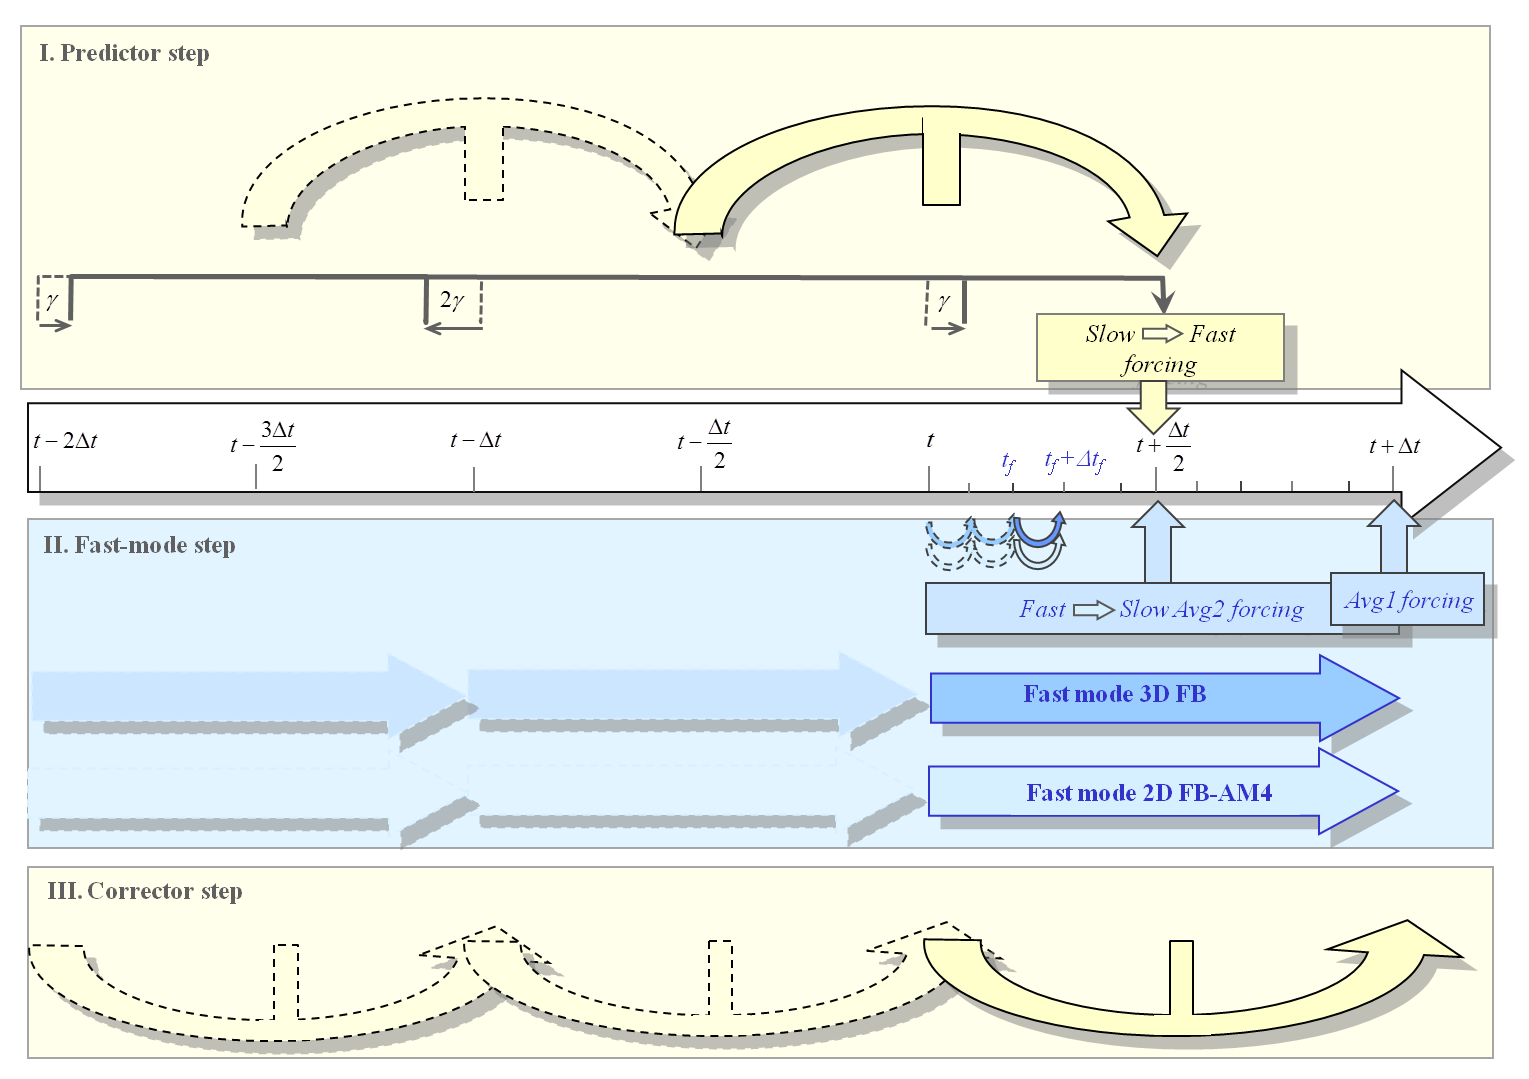
\includegraphics[width=1\linewidth]{CHAP2/Model_TS.png}
\caption[Time-splitting and time-stepping of CROCO model with its non-hydrostatic, compressible (NBQ) kernel.]{\textit{Time-splitting and time-stepping of CROCO model with its non-hydrostatic, compressible (NBQ) kernel. Yellow (blue) background color: slow (fast) kernel. }}
	\label{ModelTS}
\end{figure}
%
\begin{table}
\begin{subequations}
\label{TimeSplit}
\begin{alignat}{3}
 \displaystyle
 %%%%%%%%%%%%%%%%%%%%%%%%%%%%%%%%%%%%%%%%%%%%%%%%%%%%%%%%%%%%%
 &\nonumber \textbf{I.a Time-interpolation: } t_s-\Delta t_s/2\\[0mm]
 %%%%%%%%%%%%%%%%%%%%%%%%%%%%%%%%%%%%%%%%%%%%%%%%%%%%%%%%%%%%%
 \label{TimeSplitIa1}
 &\enspace[\Theta] ^{n-\frac{1}{2}}=\alpha_{n-1}\Theta_s^{n-1}
 +\alpha_{n}\Theta_s^{n}\\[3mm]
 %%%%%%%%%%%%%%%%%%%%%%%%%%%%%%%%%%%%%%%%%%%%%%%%%%%%%%%%%%%%%
 &\nonumber \textbf{I.b Predictor step: } t_s+\Delta t_s/2\\[0mm]
 %%%%%%%%%%%%%%%%%%%%%%%%%%%%%%%%%%%%%%%%%%%%%%%%%%%%%%%%%%%%%
 \label{TimeSplitIb1}
 &\enspace\rho h\mathbf{v}_s^{n+\frac{1}{2}}=
 \rho h\mathbf{v}_s^{n-\frac{1}{2}}
 +\Delta t_s\left(\Lambda_{s,v}^{n}+<\Lambda_{f,v}>^n\right)\\[3mm]
 %
 \label{TimeSplitIb2}
 &\enspace\rho h(\theta_s,\ S_s)^{n+\frac{1}{2}}=
 \rho h(\theta_s,\ S_s)^{n-\frac{1}{2}}
 +\Delta t_s\Lambda_{s,(\theta,S)}^{n}\\[3mm]
 %
 \label{TimeSplitIb3}
 &\enspace\rho_s^{n+\frac{1}{2}}=\rho_{eos}\left(\theta_s^{n+\frac{1}{2}},\ S_s^{n+\frac{1}{2}},\ z_s^{n+\frac{1}{2}}\right)\\[3mm]
 %
 \label{TimeSplitIb4}
 &\enspace\partial_s\rho\omega_s^{n+\frac{1}{2}}=-\partial_t\rho h_s^{n+\frac{1}{2}}
 +\mathbf{\nabla}\cdot\rho h \mathbf{u}_s^{n+\frac{1}{2}}\\[3mm]
 %%%%%%%%%%%%%%%%%%%%%%%%%%%%%%%%%%%%%%%%%%%%%%%%%%%%%%%%%%%%%
 &\nonumber \textbf{I.c AB3-extrapolation: } t_s+\Delta t_s/2\\[0mm]
 %%%%%%%%%%%%%%%%%%%%%%%%%%%%%%%%%%%%%%%%%%%%%%%%%%%%%%%%%%%%%
 \label{TimeSplitIc1}
 &\enspace[[\Psi_s]]^{n+\frac{1}{2}}=
  \beta_{n-2}\Psi_s^{n-2}
 +\beta_{n-1}\Psi_s^{n-1}
 +\beta_{n}\Psi_s^{n}\\[2mm]
 %%%%%%%%%%%%%%%%%%%%%%%%%%%%%%%%%%%%%%%%%%%%%%%%%%%%%%%%%%%%%
 &\nonumber \textbf{II. Fast-mode steps: } t_f\in(t_s,\ t_s+\Delta t_s] \textit{ or } m\in[0,\ N_f)_\mathcal{N}\\[2mm]
 %%%%%%%%%%%%%%%%%%%%%%%%%%%%%%%%%%%%%%%%%%%%%%%%%%%%%%%%%%%%%
 \label{TimeSplitIIa}
 &\enspace\zeta_f^{m+1}=\zeta_f^{m}+\Delta t_f\left(
  w_{surf}^{m}-\mathbf{u}_{surf}^{m}.\mathbf{\nabla}\zeta^{m}\right)\\[2mm]
 %
 \label{TimeSplitIIb}
 &\enspace\rho h u_f^{m+1}=
 \rho h u_f^{m}
 +\Delta t_f\left(
  [[\Lambda_{s,u}]]^{n+\frac{1}{2}}
 -[[\overline{\Lambda_{s,u}}]]^{n+\frac{1}{2}}
 +\Lambda_{f,u}^{m}
% +\overline{\overline{\Lambda_{f,u}}}^{\ m}
 +\overline{\overline{\Lambda_{f,u}}}^{\ m}
 +\overline{\overline{\Lambda_{f,-\mathbf{\nabla}\zeta}}}^{\ m+1}
 \right)\\[2mm]
 %
 \label{TimeSplitIIc}
 &\enspace\overline{\overline{\rho h U}}_f^{\ m+1}=
 \overline{\overline{\rho h U}}_f^{\ m}
 +\Delta t_f\left(
 %[[\overline{\Lambda_{s,u}}]]^{n+\frac{1}{2}}+
 \overline{\Lambda_{f,u}^{m}}
 +\overline{\overline{\Lambda_{f,u}}}^{\ m}
 +\overline{\overline{\Lambda_{f,-\mathbf{\nabla}\zeta}}}^{\ m+1}
 \right)\\[0mm]
 %
 \label{TimeSplitIId}
 &\enspace\rho h w_f^{m+1}=
 \rho h w_f^{m}
 +\Delta t_f\left([[\Lambda_{s,w}]]^{n+\frac{1}{2}}
 +\Lambda_{f,w}^{m+1*}\right)\\[2mm]
 %
 \label{TimeSplitIIe}
 &\enspace\rho h_f^{m+1}=\rho h_f^{m}
 -\Delta t_f\left(
 [[\partial_t\rho h_s]]^{n+\frac{1}{2}}
 +\mathbf{\nabla}\cdot\{\rho h \mathbf{v}\}_f^{m+1}
 \right)\\[0mm]
 %
 \label{TimeSplitIIh}
 &\enspace m=N_f-1:\ \bar{\rho}\zeta_s^{n+1}
 =\bar{\rho}(H+\zeta_f)^{m}
 -\bar{\rho}H_s^{m+1}
 -\Delta t_f\mathbf{\nabla}\cdot\overline{\overline{\rho h\mathbf{u}}}^{\ m+1}\\[2mm]
 %
 \label{TimeSplitIIg}
 &\enspace \textit{Update\ grid:}\ \rho h_f^{m+1},\ z_f^{m+1}\\[2mm]
 %
 %%%%%%%%%%%%%%%%%%%%%%%%%%%%%%%%%%%%%%%%%%%%%%%%%%%%%%%%%%%%%
 &\nonumber \textbf{III.a Filtering: } t_s+\Delta t_s\ \textit{and}\ t_s+\Delta t_s/2\\[0mm]
 %%%%%%%%%%%%%%%%%%%%%%%%%%%%%%%%%%%%%%%%%%%%%%%%%%%%%%%%%%%%%
 \label{TimeSplitIIIa1}
 &\enspace<\Phi_f>^{n+1}=\Phi_f^{m=n+1}\\[0mm]
 \label{TimeSplitIIIa2}
 &\enspace\ll\Phi_f\gg^{n+\frac{1}{2}}=\frac{1}{N_f}\sum_{m=1}^{N_f}\Phi_f^{m}\\[2mm]
 %%%%%%%%%%%%%%%%%%%%%%%%%%%%%%%%%%%%%%%%%%%%%%%%%%%%%%%%%%%%%
 &\nonumber \textbf{III.b Corrector step: } t_s+\Delta t_s\\[0mm]
 %%%%%%%%%%%%%%%%%%%%%%%%%%%%%%%%%%%%%%%%%%%%%%%%%%%%%%%%%%%%%
 %
 \label{TimeSplitIIIb1}
 &\enspace\rho h\mathbf{v}_s^{n+1}=
 \rho h\mathbf{v}_s^{n}
 +\Delta t_s\left(\Lambda_s^{n+\frac{1}{2}*}
 +\ll\Lambda_f\gg^{n+\frac{1}{2}}\right)\\[0mm]
 %
 \label{TimeSplitIIIb2}
 &\enspace\partial_s\rho\omega_s^{n+1}=
 -\partial_{t\ }\rho h_s^{n+1}
 +\mathbf{\nabla}\cdot\rho h \mathbf{u}_s^{\ n+1}
 -\overline{\mathbf{\nabla}\cdot\rho h \mathbf{u}_s}^{\ n+1}
 -\overline{<\mathbf{\nabla}\cdot\rho h \mathbf{u}_s>}^{\ n+1}\\[2mm]
 %
 \label{TimeSplitIIIb3}
 &\enspace\rho h(\theta_s,\ S_s)^{n+1}=
 \rho h(\theta_s,\ S_s)^{n}
 +\Delta t_s\Lambda_{s,(\theta,S)}^{n+\frac{1}{2}*}\\[0mm]
 %
 \label{TimeSplitIIIb4}
 &\enspace\rho_s^{n+1}=\rho_{eos}\left(\theta_s^{n+1},\ S_s^{n+1},\ z_s^{n+1}\right)\\[0mm]
 %
 \label{TimeSplitIIIb5}
 &\enspace\rho h\mathbf{u}_s^{n+1}=\rho h\mathbf{u}_s^{n+1}
 -\overline{\rho h\mathbf{u}_s}^{\ n+1}
 +\overline{\rho h\mathbf{u}_f}^{\ m=N_f-1}
 %%%%%%%%%%%%%%%%%%%%%%%%%%%%%%%%%%%%%%%%%%%%%%%%%%%%%%%%%%%%%
\end{alignat}
\end{subequations}
\end{table}
Predictor (I), fast-kernel Forward-Backward (II) and Corrector (III) steps are shown in horizontal color bands on Figure \noparref{ModelTS} (yellow for the slow kernel, blue for the fast kernel). After time-interpolating slow-kernel variables to $t_s-\Delta t_s/2$ (step I.a, notation $[.]$), the slow kernel is advanced from $t_s-\Delta t_s/2$ to $t_s+\Delta t_s/2$ with a centered, leap-frog-like, time-stepping (step I.b). Then, to prepare the integration of the fast kernel, the slow-kernel RHS is extrapolated to $t_s+\Delta t_s/2$ based on an AB3 scheme using its previous evaluations at $t_s-2\Delta t_s$, $t_s-\Delta t_s$ and $t_s$ (step I.c, notation $[[.]]$). The fast kernel can in turn be advanced from $t_s$ to $t_s+\Delta t_s$ using a forward-backward like time-stepping (step II) with time-step $\Delta t_f$ satisfying  $N_f=\Delta t_s/\Delta t_f\in\mathcal{N}$. The vertical momentum equation can optionally be integrated with semi-implicit scheme over the vertical direction.

The vertical grid is updated at each fast time-step (Equation \noparref{TimeSplitIIg}) but slow-kernel components of the RHS remain constant during the fast-kernel integration. At the last fast time-step, surface elevation displacement for the slow kernel can be recomputed to ensure perfect numerical coherence between the surface kinematic relation and depth-integrated mass conservation (Equations \noparref{TimeSplitIIa} and \noparref{TimeSplitIIh}).

Further numerical details such as the values of the interpolation $(\alpha_n)$ or extrapolation $(\beta_n)$ coefficients, the expressions of the slow-kernel RHS terms $(\Lambda_s)$, the expressions of the fast-kernel surface-related pressure force terms $(\Lambda_{f,-\nabla\zeta})$,  the fast-kernel RHS remaining terms $(\Lambda_{f})$ or the implicit fast and slow-kernel RHS terms (indicated by an asterisk) can be found in CROCO dedicated manuals and publications. 
A major difference with the hydrostatic time-splitting is that the surface elevation displacement is given by the kinematic condition (Equation \noparref{TimeSplitIIa}) and not by the depth-integral of the mass conservation equation. Once the fast-kernel RHS and variables have been filtered both at $t_s+\Delta t_s$ and $t_s+\Delta t_s/2$ (step III.a, notations $<.>$ and $\ll.\gg$), the slow kernel is finally advanced from $t$ to  $t_s+\Delta t_s$ during the leap-frog-like Corrector step (III.b). A star following the time-index superscript indicates the use of an implicit numerical schemes.

Note that the 2D depth-averaged, barotropic-like, horizontal momentum Equations \noparref{TimeSplitIIc} (double over-bar notation) are advanced in the same way as in \cite{shchepetkin_regional_2005}. The result of this 2D integration is indeed used to correct both the horizontal momentum itself and the RHS of the horizontal momentum equation at Corrector step. It can also be used to require a perfect coherence of the surface elevation displacement and the depth-average transport (at machine precision) during the slow-mode integration.


\section{Conclusion, discussion of the \textit{ocean model}}
In the present chapter, we proposed a rigorous framework (a "map") for our exploration of ocean \textit{fine scales} in the \textit{Terra Incognita}. An analytical, terrain-following s-coordinate model for the conservation of mass, momentum, heat and tracers has first been proposed under general assumptions of a compressible, free-surface ocean (\S \noparref{section_prim_eq}). 

We then considered the numerical implementation of this general \textit{ocean model} (\S \noparref{section_croco}). After a consideration of the space-time scales potentially involved in fine scale ocean dynamics, an original time-splitting has been detailed as an extension of \cite{shchepetkin_regional_2005}'s barotropic/baroclinic time-splitting. It is also a restriction to a two-mode time-splitting of \cite{Auclair2018}'s three-mode time-splitting. This time-splitting allows the integration of both acoustic and surface-induced processes with a smaller time-step in order to make the integration of a compressible, free-surface realistic ocean affordable. It is based on the spectral gaps identified in Equation \noparref{velocityscales} between acoustic, surface and internal processes.

The region of the Strait of Gibraltar has been chosen as the region of demonstration for fine-scale dynamics in CROCO. As a consequence, the LES configurations presented in Chapters \noparref{chapGBR2D}, \noparref{chapGBR3D} and \noparref{chapBPE} are not only based on the two-mode CROCO kernel of Section \noparref{section_croco}; these configurations have indeed been part of the development process itself. 


%%%%%%%%%%%%%%%%%%%%%%%%%%%%%%%%%%%%%%%%%%%%%%%%%%%%%%%%%%%%%%%%%%%%%%%%%%%
\section{Appendices to the \textit{ocean model}}
\label{annexe_ocmod}
%%%%%%%%%%%%%%%%%%%%%%%%%%%%%%%%%%%%%%%%%%%%%%%%%%%%%%%%%%%%%%%%%%%%%%%%%%%
%%%%%%%%%%%%%%%%%%%%%%%%%%%%%%%%%%%%%%%%%%%%%%%%%%%%

\subsection{$s$-coordinate transformation}
\label{section_annexe2}
The present appendix gathers several formula and relations essential to the development of the numerical implementation of the \textit{ocean model}.
%
%%%%%%%%%%%%%%%%%%%%%%%%%%%%%%%%%%%%%%%%%%%%%%%%%%%%%%%%%%%%%%%%%%%%%%%%%%%%%
\subsubsection{Transformation matrices}
\label{annexe_coordS}
%%%%%%%%%%%%%%%%%%%%%%%%%%%%%%%%%%%%%%%%%%%%%%%%%%%%%%%%%%%%%%%%%%%%%%%%%%%%%
The transformation matrix of the generalized coordinate transformation is:
\begin{equation}
    \displaystyle
    \Lambda^z_s=
    \begin{pmatrix}
    1 & 0 & 0 & 0 \\
    0 & 1 & 0 & 0 \\
    0 & 0 & 1 & 0 \\
    \frac{\partial z}{\partial t} & \frac{\partial z}{\partial x}
    & \frac{\partial z}{\partial y} & h=\frac{\partial z}{\partial s}
    \end{pmatrix}
\end{equation}
and the inverse transformation is given by:
\begin{equation}
    \displaystyle
    \Lambda_z^s=
    \begin{pmatrix}
    1 & 0 & 0 & 0 \\
    0 & 1 & 0 & 0 \\
    0 & 0 & 1 & 0 \\
    \frac{\partial s}{\partial t} & \frac{\partial s}{\partial x}
    & \frac{\partial s}{\partial y} & \frac{\partial s}{\partial z}
    \end{pmatrix}
\end{equation}
The Jacobian of the transformation $J=det(\Lambda^z_s)$ is the (specific) thickness:
\begin{equation}
 \displaystyle
 J=h=\frac{\partial z}{\partial s}=\frac{\partial z}{\partial s}\bigg\vert_{xyt}
\end{equation}
\cite{griffies_fundamentals_2004} further define the infinitesimal  thickness for modelling developments:
\begin{equation}
 \displaystyle
 \delta h=\frac{\partial z}{\partial s} \delta s
\end{equation}

%%%%%%%%%%%%%%%%%%%%%%%%%%%%%%%%%%%%%%%%%%%%%%%%%%%%%%%%%%%%%%%%%%%%%%%%%%%%%
\subsubsection{Formula and identities}
%%%%%%%%%%%%%%%%%%%%%%%%%%%%%%%%%%%%%%%%%%%%%%%%%%%%%%%%%%%%%%%%%%%%%%%%%%%%%
Base on the transformation matrices, the $s$-coordinate transformations can be rewritten:
\begin{subequations}
  \begin{alignat}{2}
  \displaystyle 
  &\frac{\partial A}{\partial t}\bigg\rvert_{xz} &&=
   \frac{\partial A}{\partial t}\bigg\rvert_{xs}
  - \frac{1}{h} \frac{\partial A}{\partial s}\bigg\rvert_{tx}
  \frac{\partial z}{\partial t}\bigg\rvert_{xs}\\[4mm]
  &\frac{\partial A}{\partial x}\bigg\rvert_{tz} &&=
   \frac{\partial A}{\partial x}\bigg\rvert_{ts}
  - \frac{1}{h} \frac{\partial A}{\partial s}\bigg\rvert_{tx}
  \frac{\partial z}{\partial x}\bigg\rvert_{ts}\\[4mm]
  &\frac{\partial A}{\partial z}\bigg\rvert_{tx} &&=
   \frac{1}{h}
   \frac{\partial A}{\partial s}\bigg\rvert_{tx}
  \end{alignat}
\end{subequations}
whereas material derivatives satisfy:
\begin{subequations}
  \begin{alignat}{2}
  \displaystyle 
  & \frac{d}{dt} &&=\frac{\partial}{\partial t}\bigg\vert_z
  + \mathbf{u}.\mathbf{\nabla}_z
  + w\frac{\partial }{\partial z}\\[4mm]
  & &&=\frac{\partial}{\partial t}\bigg\vert_s
  + \mathbf{u}.\mathbf{\nabla}_s
  + \dot{s}\frac{\partial}{\partial s}
  \end{alignat}
\end{subequations}
This leads to:
\begin{equation}
  \displaystyle 
  \dot{z} =\frac{dz}{dt}\bigg\vert_s=\frac{\partial z}{\partial t}\bigg\vert_s
  + \mathbf{u}.\mathbf{\nabla}_s z
  + \dot{s}\frac{\partial z}{\partial s},\quad r\quad
  \dot{s} =\frac{ds}{dt}\bigg\vert_z=\frac{\partial s}{\partial t}\bigg\vert_z
  + \mathbf{u}.\mathbf{\nabla}_z s
  + w\frac{\partial s}{\partial z}
\end{equation}
Using the identities:
\begin{equation}
  \displaystyle
  \frac{\partial s}{\partial t}\bigg\vert_z =
  \left(\frac{\partial t}{\partial s}\bigg\vert_z\right)^{-1},\quad
  \frac{\partial s}{\partial x}\bigg\vert_z =
  \left(\frac{\partial x}{\partial s}\bigg\vert_z\right)^{-1},\quad
  \frac{\partial s}{\partial y}\bigg\vert_z =
  \left(\frac{\partial y}{\partial s}\bigg\vert_z\right)^{-1},\quad
  \frac{\partial s}{\partial z}\bigg\vert_x =
  \left(\frac{\partial z}{\partial s}\bigg\vert_x\right)^{-1}
\end{equation}
several relations can be obtained from the triple product rule and the coordinate transformations are given by:
\begin{equation}
  \displaystyle
  \frac{\partial z}{\partial t}\bigg\vert_s =
  -\frac{\partial s}{\partial t}\bigg\vert_z\frac{\partial z}{\partial s}\bigg\vert_s,\quad
  \frac{\partial z}{\partial x}\bigg\vert_s =
  -\frac{\partial s}{\partial x}\bigg\vert_z\frac{\partial z}{\partial s}\bigg\vert_s,\quad
  \frac{\partial z}{\partial y}\bigg\vert_s =
  -\frac{\partial s}{\partial y}\bigg\vert_z\frac{\partial z}{\partial s}\bigg\vert_s\\
\end{equation}

%%%%%%%%%%%%%%%%%%%%%%%%%%%%%%%%%%%%%%%%%%%%%%%%%%%%%%%%%%%%%%%%%%%%%%%%%%%%%
\subsubsection{Local orthonormal coordinates}
%%%%%%%%%%%%%%%%%%%%%%%%%%%%%%%%%%%%%%%%%%%%%%%%%%%%%%%%%%%%%%%%%%%%%%%%%%%%%
\cite{griffies_fundamentals_2004} further defines in his chapter (6.4) a system of orthonormal coordinates:
\begin{equation}
  \displaystyle 
  \mathbf{e}_{x^*} =\frac{\mathbf{y}\wedge{\mathbf{\nabla}s}}
  {\norm{\mathbf{y}\wedge{\mathbf{\nabla}s}}},\quad
  \mathbf{e}_{y^*} =\mathbf{e}_s\wedge{\mathbf{e}_{x^*}},\quad
  \mathbf{e}_s =\frac{\mathbf{\nabla}s}{\norm{\mathbf{\nabla}s}}
\end{equation}
In this particular case ($\mathbf{e}_s.\mathbf{z}$) has a unique sign, the basis vectors can be rewritten:
\begin{equation}
  \displaystyle 
  \mathbf{e}_{x^*} =\frac{\mathbf{x}+S_x\mathbf{z}}{\sqrt{1+S_x^2}},\quad
  \mathbf{e}_{y^*} =\frac{-S_xS_y\mathbf{x}+(1+S_x^2)\mathbf{y}+S_y\mathbf{z}}{\sqrt{1+S^2)(1+S_x^2)}},\quad
  \mathbf{e}_s =\frac{(-\mathbf{S},1)}{\sqrt{1+S^2}}
\end{equation}
The s-coordinate transformation is a rotation and:
\begin{equation}
   \displaystyle
   \mathbf{e}_{x^*y^*s}=\Lambda_{s}^{z}\mathbf{e}_{xyz}
\end{equation}
Note in particular the definition of the slope $\mathbf{S}$ and its norm $S=\norm{\mathbf{S}}$ used to rewrite the orthonormal basis:
\begin{equation}
   \displaystyle
   \mathbf{S}=\mathbf{\nabla}_s z=
   -\frac{\partial z}{\partial s}\mathbf{\nabla}_z s=\left( S_x,\ S_y,\ 0 \right)
\end{equation}
where $\mathbf{\nabla}_s z$ is "the horizontal gradient of the height of a fluid parcel as taken along surfaces of constant generalized vertical coordinate s" \citep{griffies_fundamentals_2004}.

Note that this orthonormal basis is not used to project the equations of the model. S-coordinates are "only" used as a change of variable whereas equations and vector quantities remain written in the original Cartesian or spherical basis. The present s-coordinate orthonormal basis is presented here to be latter used in the computation of fluxes through s-surfaces.


%%%%%%%%%%%%%%%%%%%%%%%%%%%%%%%%%%%%%%%%%%%%%%%%%%%%%%%%%%%%%%%%%%%%%%%%%%%%%
\subsection{Operators \& relations in s-coordinates}
\label{annexe_s-coord}
%%%%%%%%%%%%%%%%%%%%%%%%%%%%%%%%%%%%%%%%%%%%%%%%%%%%%%%%%%%%%%%%%%%%%%%%%%%%%

%%%%%%%%%%%%%%%%%%%%%%%%%%%%%%%%%%%%%%%%%%%%%%%%%%%%%%%%%%%%%%%%%%%%%%%%%%%%%
\subsubsection{Divergence of the velocity field in s-coordinates}
%%%%%%%%%%%%%%%%%%%%%%%%%%%%%%%%%%%%%%%%%%%%%%%%%%%%%%%%%%%%%%%%%%%%%%%%%%%%%
Using :
\begin{equation}
 \displaystyle
 \frac{\partial}{\partial t} \frac{\partial z}{\partial s}\bigg\vert_{tx}= \frac{\partial h}{\partial t} \qquad and \qquad \frac{\partial}{\partial x} \frac{\partial z}{\partial s}\bigg\vert_{tx}= \frac{\partial h}{\partial x}
\end{equation}
%and
%\begin{equation}
% \displaystyle
% \frac{\partial}{\partial x} \frac{\partial z}{\partial s}\bigg\vert_{tx}= \frac{\partial h}{\partial x}
%\end{equation}
%
the expression of the divergence of the velocity field in s-coordinates can be written:
\begin{subequations}
  \begin{alignat}{2}
  & h \ \mathbf{\nabla}.( \mathbf v) &&= h \frac{\partial u}{\partial x} \bigg \rvert_{zt} +h \frac{\partial v_z}{\partial z} \bigg \rvert_{xt}\\[4mm]
  & && = h \frac{\partial u}{\partial x} \bigg \rvert_{st} - \frac{h}{h} \frac{\partial u}{\partial s}\bigg \rvert_{tx} \frac{\partial z}{\partial x}\bigg \rvert_{ts}
  \quad + \frac{h}{h}  \frac{\partial}{\partial s} \bigg ( v_s + \frac{\partial z }{\partial t}\bigg \rvert_{xs} + u \frac{\partial z}{\partial x}\bigg \rvert_{ts} \bigg )\\[4mm]
  & && = h \frac{\partial u}{\partial x} \bigg \rvert_{st} -  \frac{\partial u}{\partial s}\bigg \rvert_{tx} \frac{\partial z}{\partial x}\bigg \rvert_{ts} 
  \quad +  \frac{\partial v_s}{\partial s} +  \frac{\partial h}{\partial t} + u \frac{\partial h}{\partial x} + \frac{\partial u}{\partial s}\bigg \rvert_{tx} \frac{\partial z}{\partial x}\bigg \rvert_{ts}\\[4mm]
  & && = \frac{\partial v_s}{\partial s}\bigg \rvert_{tx} + \frac{\partial h u}{\partial x} \bigg \rvert_{ts}+ \frac{\partial h}{\partial t}\bigg \rvert_{xs}
  \end{alignat}
\end{subequations}
Note that this is a particular case of the formulation of a change of variables with its Jacobian ($J=h$ in the present case). %This leads to several useful conservative formulations in the following section.
%
%%%%%%%%%%%%%%%%%%%%%%%%%%%%%%%%%%%%%%%%%%%%%%%%%%%%%%%%%%%%%%%%%%%%%%%%%%%%%
\subsubsection{Conservative "flux" forms: kinematics \& dynamics}
%%%%%%%%%%%%%%%%%%%%%%%%%%%%%%%%%%%%%%%%%%%%%%%%%%%%%%%%%%%%%%%%%%%%%%%%%%%%%
Two general conservative formulations can be obtained combining this with the continuity equation \citep{auclair_woceanfr_2011}\footnote{WOcean.fr Web Site: \url{http://poc.omp.obs-mip.fr/auclair/WOcean.fr/SNH/Restricted/NH-NBQ/Sources/Images/png/Coord_demo.png}\label{WOcean_scoord}}.

$A$ is a property given per unit mass (thermodynamically intensive) (see the demonstration on web site). The first two (conservative) relations are fundamentals to analytical and numerical modeling.


\textbf{\textit{Based on the conservation of mass:}}
\begin{equation}
  \displaystyle 
  \rho \frac{d A}{dt}
  =\frac{\partial \rho A}{\partial t}\bigg\rvert_{xz}
  +\frac{\partial \rho A u}{\partial x}\bigg\rvert_{tz}
  +\frac{\partial \rho  v_s}{\partial z}\bigg\rvert_{tx}
\end{equation}

\textbf{\textit{Based on the conservation of mass \& in s-coordinates:}}
\begin{equation}
  \displaystyle 
  \rho h \frac{d A}{dt}
  =\frac{\partial \rho h A}{\partial t}\bigg\rvert_{xs}
  +\frac{\partial \rho h A u}{\partial x}\bigg\rvert_{ts}
  +\frac{\partial \rho  A v_s}{\partial s}\bigg\rvert_{tx}
\end{equation}
\textbf{\textit{A kinematic, non-conservative formulation}} can be obtained without the continuity equation:
\begin{equation}
\frac{d A}{d t} = \frac{\partial A}{\partial t} \bigg\rvert_{xs} + u \frac{\partial A}{\partial x} \bigg\rvert_{ts} + \frac{v_s}{h}\frac{\partial A}{\partial s}\bigg\rvert_{tx}
\end{equation}
The demonstration is given in \citep{auclair_woceanfr_2011}$^{\noparref{WOcean_scoord}}$.\\

\textbf{\textit{Conservation of mass:}}
note finally that the conservation of mass $A=1$ can then be rewritten:
\begin{equation}
  \displaystyle 
  \label{mass_s}
  h\frac{d\rho}{d t}
  =\frac{\partial \rho h }{\partial t}\bigg\rvert_{xs}
  +\frac{\partial \rho h u}{\partial x}\bigg\rvert_{ts}
  +\frac{\partial \rho  v_s}{\partial s}\bigg\rvert_{tx}
\end{equation}

Additionally, the evolution of $\rho$ in Equation \noparref{eq_diff_cart} can be rewritten in s-coordinates as:
\begin{equation}
\label{eq_diff_s}
\displaystyle
h \frac{d \rho }{d t} \approx
\frac{\partial}{\partial x} \bigg(h \kappa^h \frac{\partial \rho}{\partial x}\bigg\rvert_{ts}\bigg)_{ts}
+ \frac{\partial}{\partial s} \bigg(\frac{\kappa^v}{h} \frac{\partial \rho}{\partial s}\bigg\rvert_{tx}\bigg)_{tx} 
\end{equation}
with: $\kappa_c^h \approx \kappa^h$ and $\kappa_c^v \approx \kappa^v$.\\
